\documentclass[12pt,a4paper]{article}
\usepackage{geometry}
\usepackage[numbers]{natbib}
\usepackage{amssymb, amsmath}
\usepackage{graphicx}
\usepackage{grffile}
\graphicspath{{../Figures/}}
\usepackage{gensymb}
\usepackage[font=small]{caption}
\usepackage[utf8]{inputenc}
\usepackage[english]{babel}
\usepackage{fancyhdr}
\usepackage[raggedright]{titlesec}
\usepackage{subcaption}
\usepackage{multirow}
\usepackage{dirtytalk}
\usepackage{framed}
\usepackage[normalem]{ulem}
\usepackage[pdftex,breaklinks]{hyperref}
\hypersetup{
  colorlinks   = true, %Colours links instead of ugly boxes
  urlcolor     = green, %Colour for external hyperlinks
  linkcolor    = blue, %Colour of internal links
  citecolor   = red %Colour of citations
}


\begin{document}
\author{Katrina Ashton}


\pagestyle{fancy}
\fancyhf{}
\rhead{\thepage}
\lhead{u5586882}

\section{What I've done}
\begin{itemize}
  \item Used MATLAB do regsitration with ICP
  \item Tried to do some more investigations into what cause the bad depth estimates (angle, distance, speed). But the timestamps didn't record properly.
\end{itemize}

\section{Parts of report to look at}
\begin{itemize}
\item 
\end{itemize}

\section{Questions}
\begin{itemize}
\item 
\end{itemize}

\section{Comments}
\begin{itemize}
  \item The MATLAB registration did not work very well. It was also very fiddly to find processing frequencies where the registration wouldn't throw an error. I also ended up having to downsample the point clouds to get it to work (and because otherwise it was very slow). I might be able to get something that's less terrible by trying different frequencies to find one that works without downsampling. But I doubt the results will be particularly good, and it will be very slow.
  \item The timestamps for the depth measurements of the last few rosbags I've recorded haven't been working properly (wrong timestamps, the RGB ones seem to be fine though).
\end{itemize}

  % \begin{figure}[b!]
  %   \begin{subfigure}[t]{\textwidth}
  %   \centering
  %     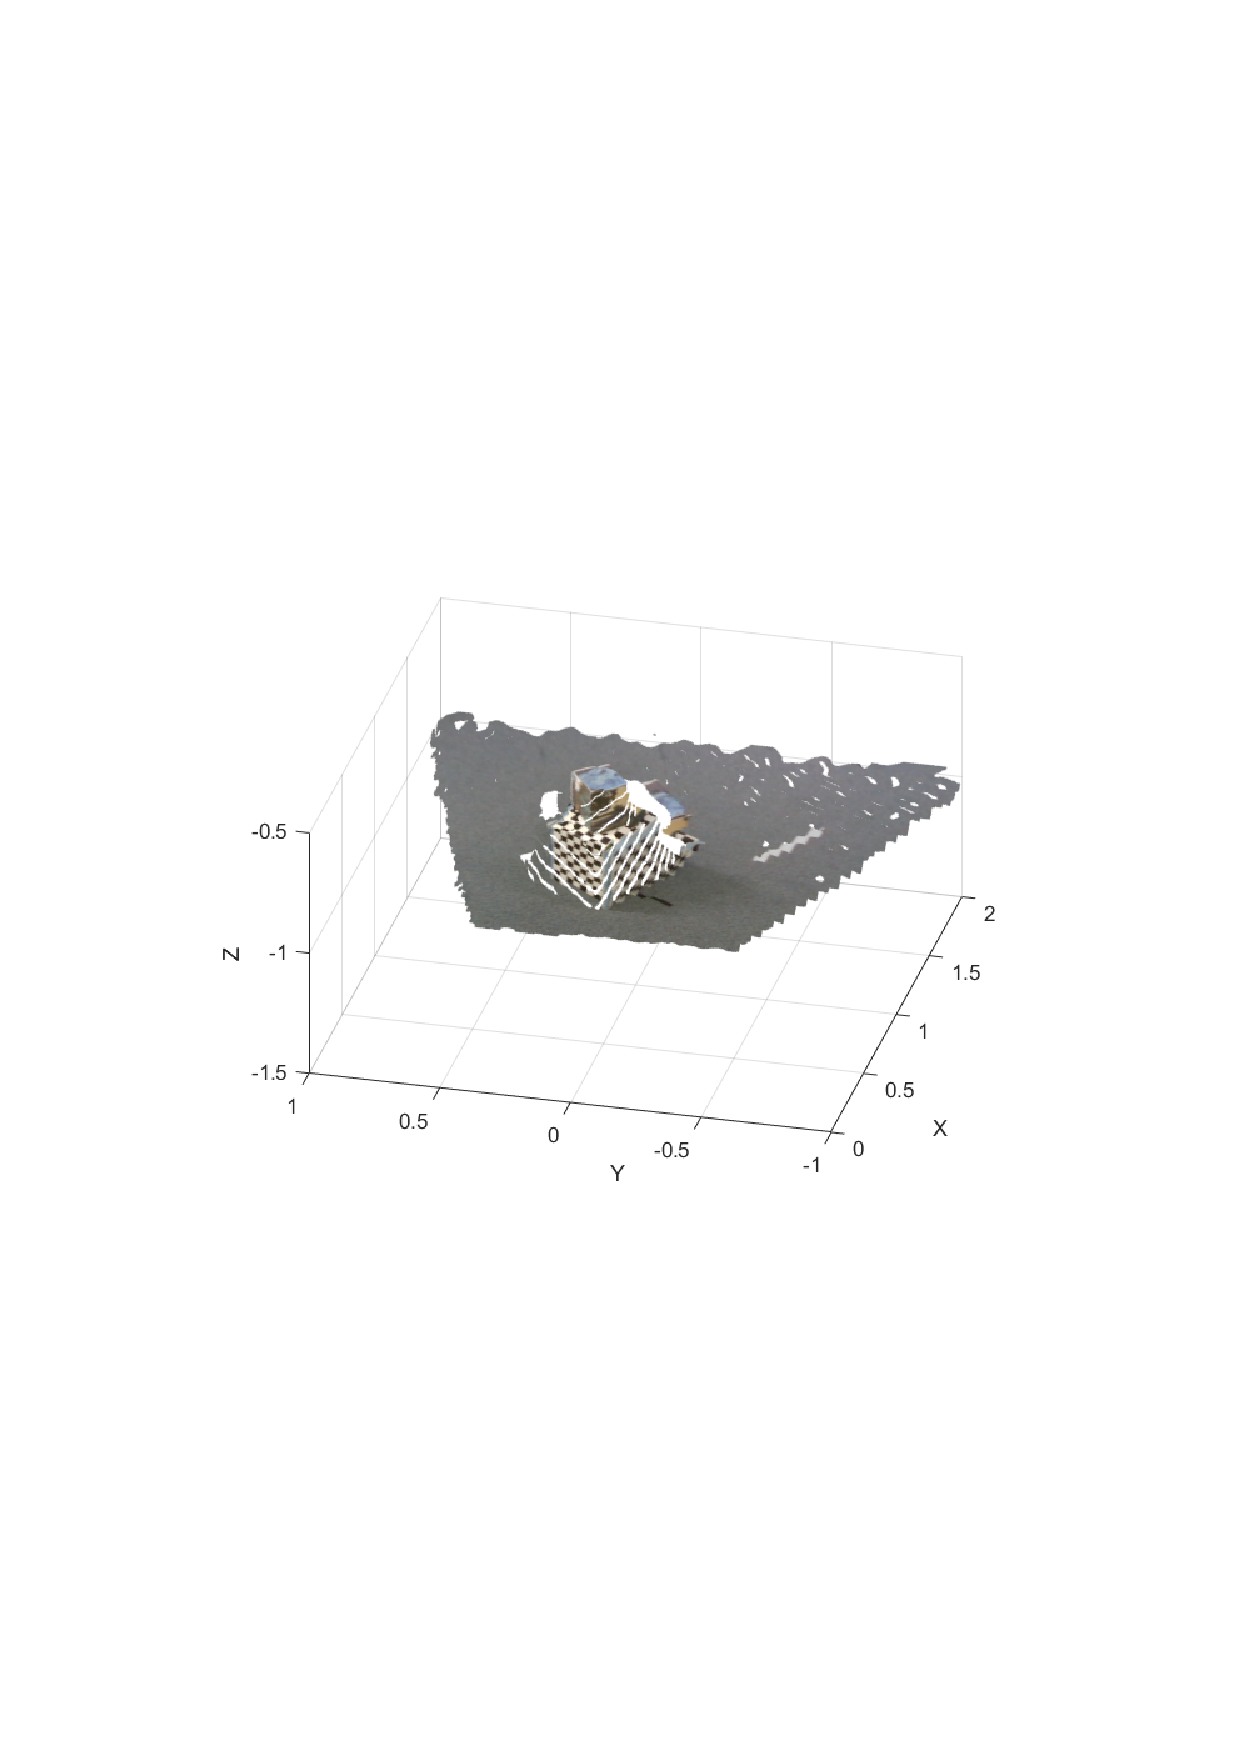
\includegraphics[width=80mm, trim = 100 280 100 290, clip]{pc_investigation/MATLAB_a.pdf}
  %     \caption{Example point cloud taken from RealSense attached to quadcopter}
  %     \label{f: pcs quad}
  %   \end{subfigure}  \\
  %   \begin{subfigure}[t]{0.5\textwidth}
  %     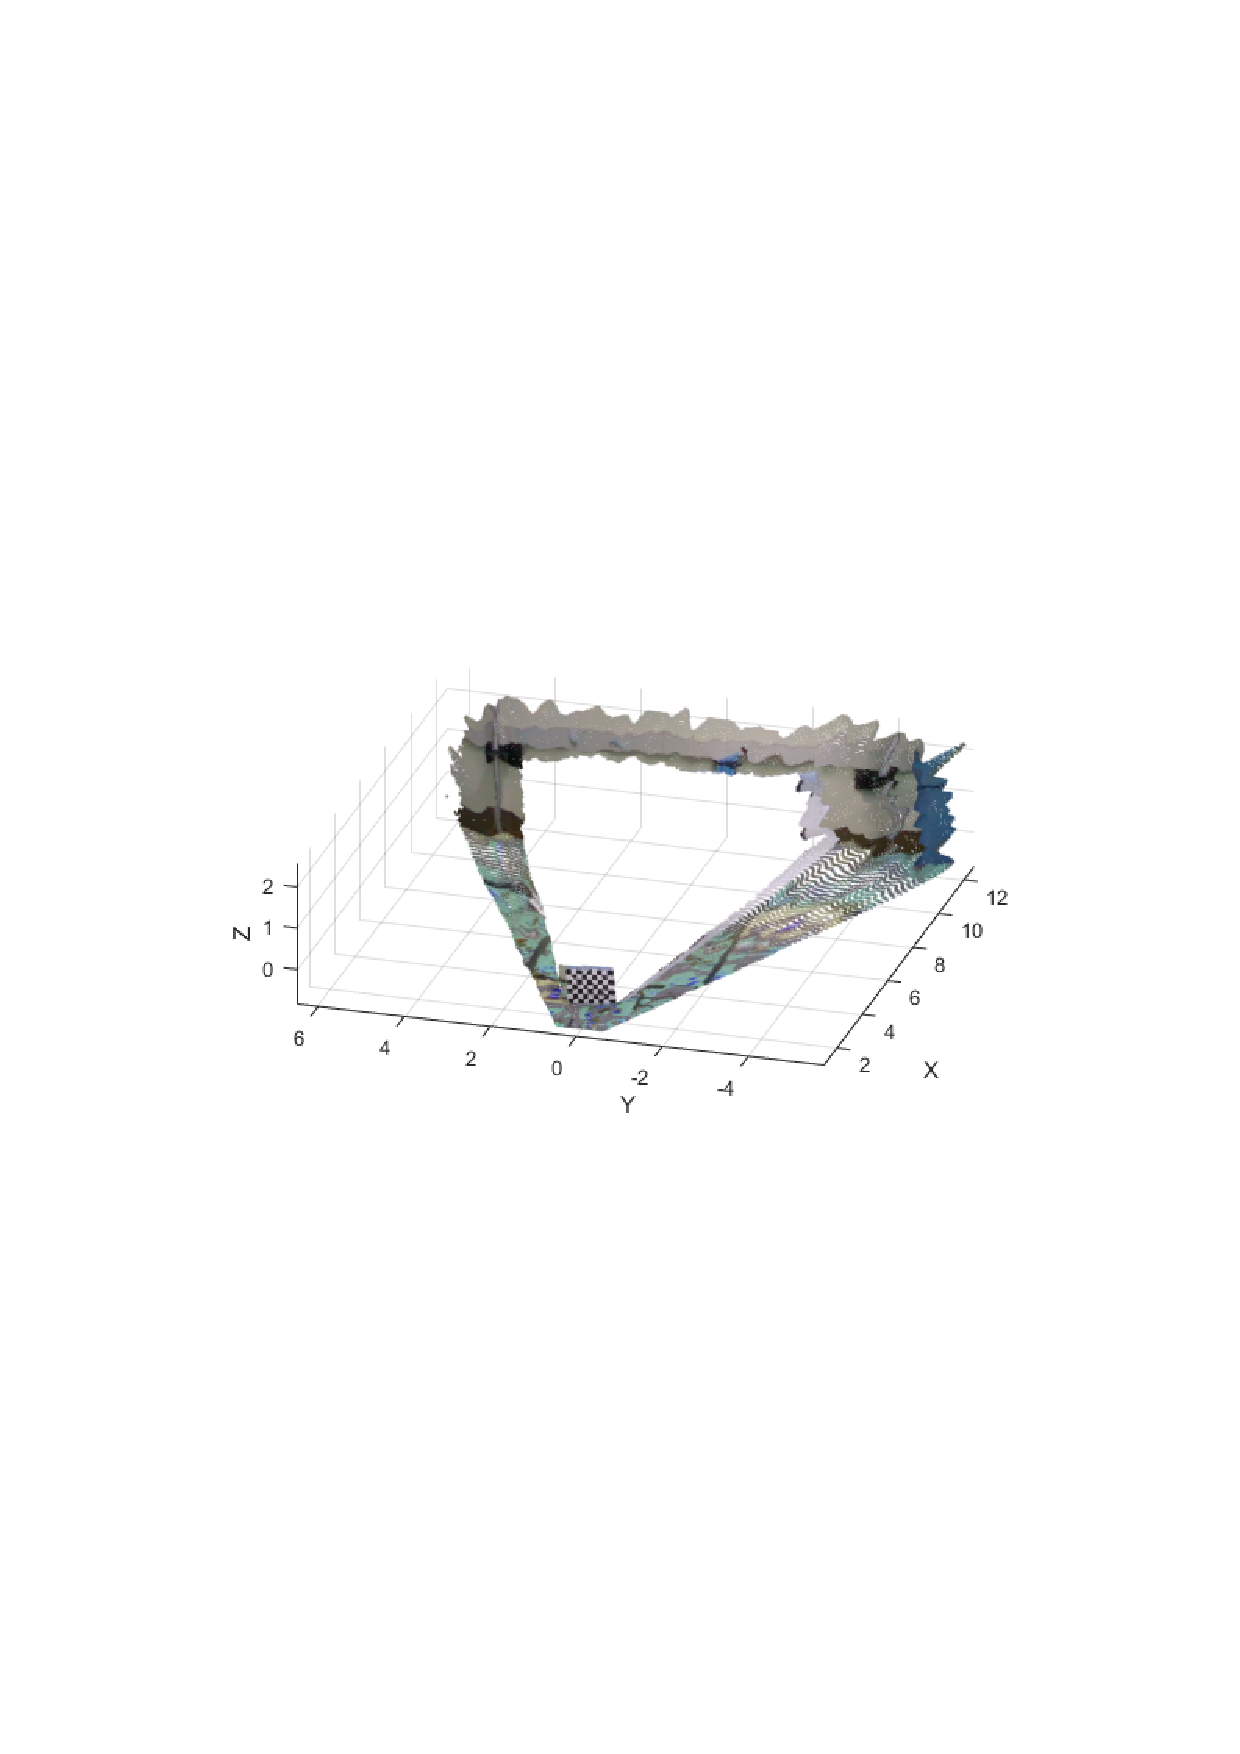
\includegraphics[width=80mm, trim = 100 300 100 290, clip]{vicon_test/without.pdf}
  %     \caption{Point cloud taken of scene from still RealSense camera, without Vicon on}
  %   \end{subfigure} %
  %   ~
  %   \begin{subfigure}[t]{0.5\textwidth}
  %   \centering
  %     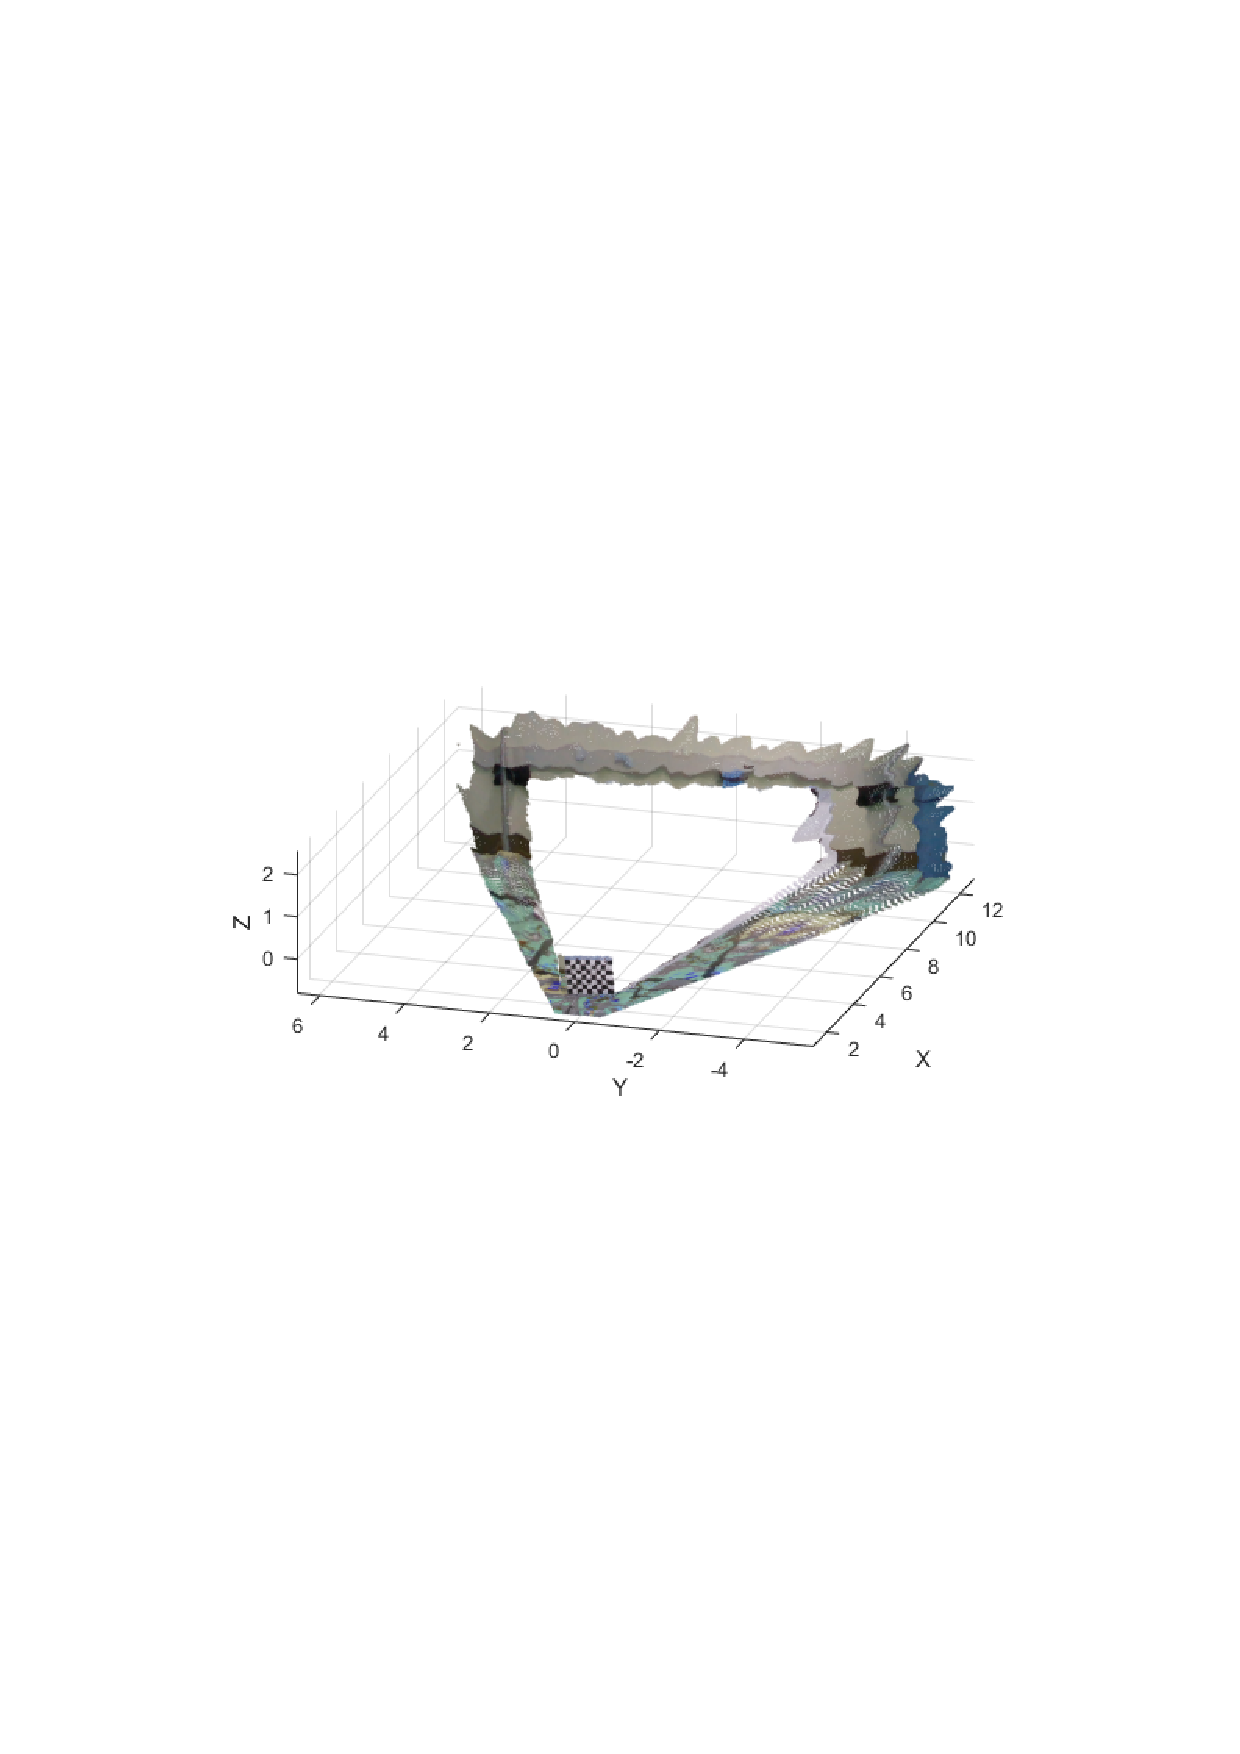
\includegraphics[width=80mm, trim = 100 300 100 290, clip]{vicon_test/with.pdf}
  %     \caption{Point cloud taken of scene from still RealSense camera, with Vicon on}
  %   \end{subfigure} 
  %   \caption{Investigating soures of error in depth measurements via visualizing point clouds. Note that all point clouds have been aligned with the quadcopter-fixed frame.}
  %   \label{f: pcs}
  % \end{figure}

    \begin{figure}[b!]
      \begin{subfigure}[t]{0.5\textwidth}
      \centering
        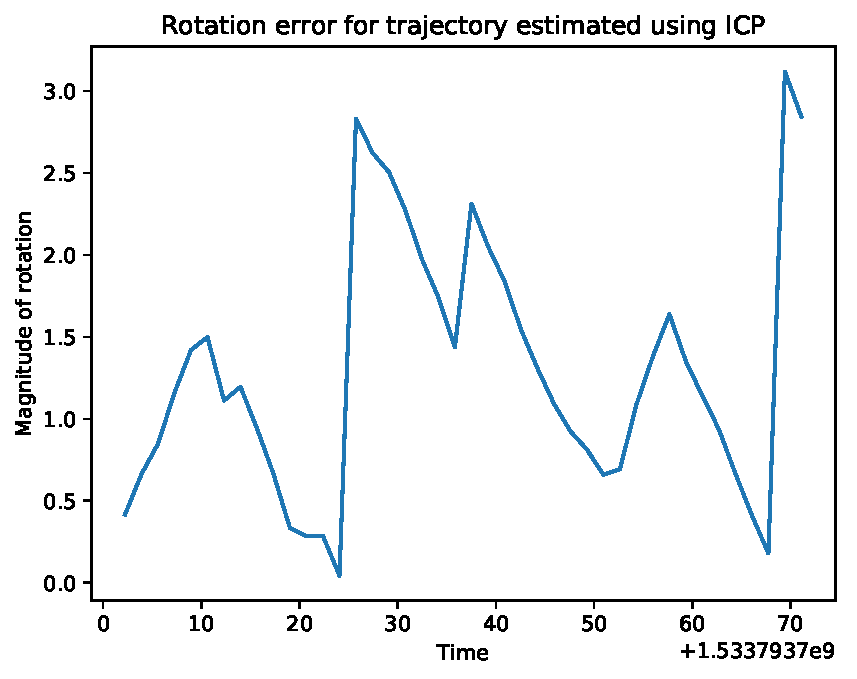
\includegraphics[width=80mm]{../quad/basic-reg-saves/50/aeR_icp.pdf}
        \caption{Absolute rotation error}
      \end{subfigure} %
      ~
      \begin{subfigure}[t]{0.5\textwidth}
        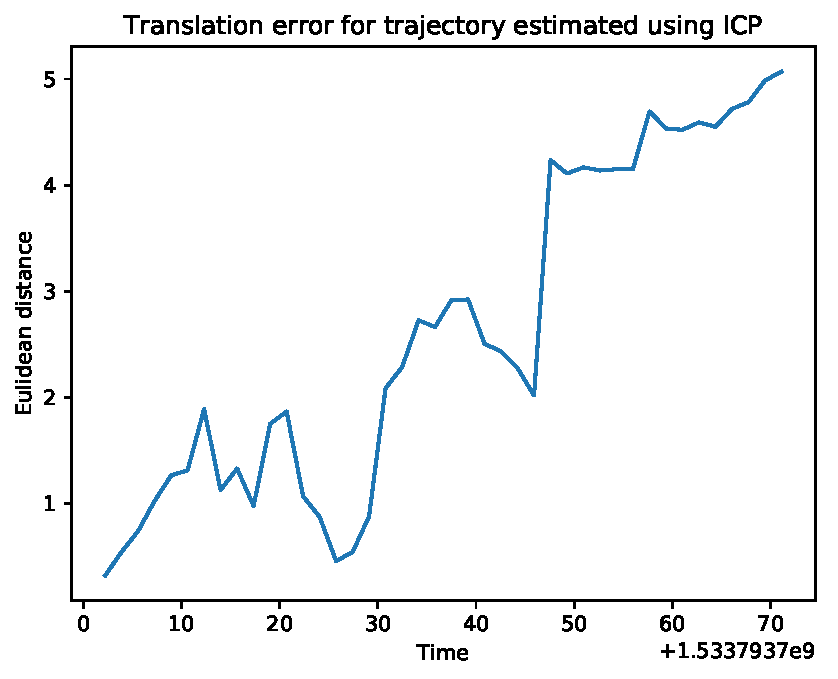
\includegraphics[width=80mm]{../quad/basic-reg-saves/50/aet_icp.pdf}
        \caption{Absolute translation error}
      \end{subfigure} \\
      \begin{subfigure}[t]{0.5\textwidth}
      \centering
        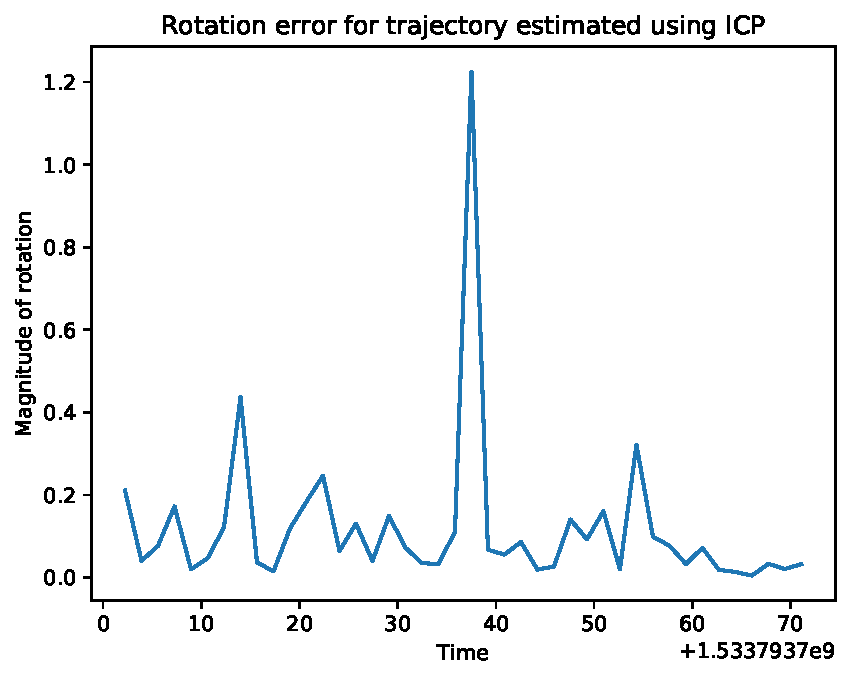
\includegraphics[width=80mm]{../quad/basic-reg-saves/50/reR_icp.pdf}
        \caption{Relative rotation error}
      \end{subfigure} %
      ~
      \begin{subfigure}[t]{0.5\textwidth}
        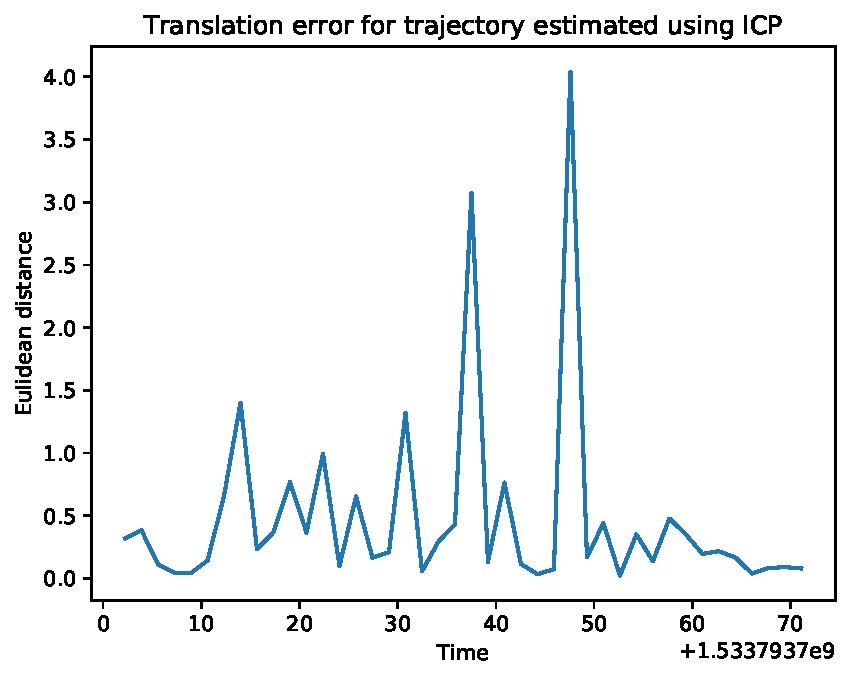
\includegraphics[width=80mm]{../quad/basic-reg-saves/50/ret_icp.pdf}
        \caption{Relative translation error}
      \end{subfigure}
      \caption{Registration error for ICP on the quadcopter 1 dataset, with 50 frames skipped.}
      \label{f: quad3 error}
    \end{figure}

     \begin{figure}[p]
      \begin{subfigure}[t]{\textwidth}
      \centering
        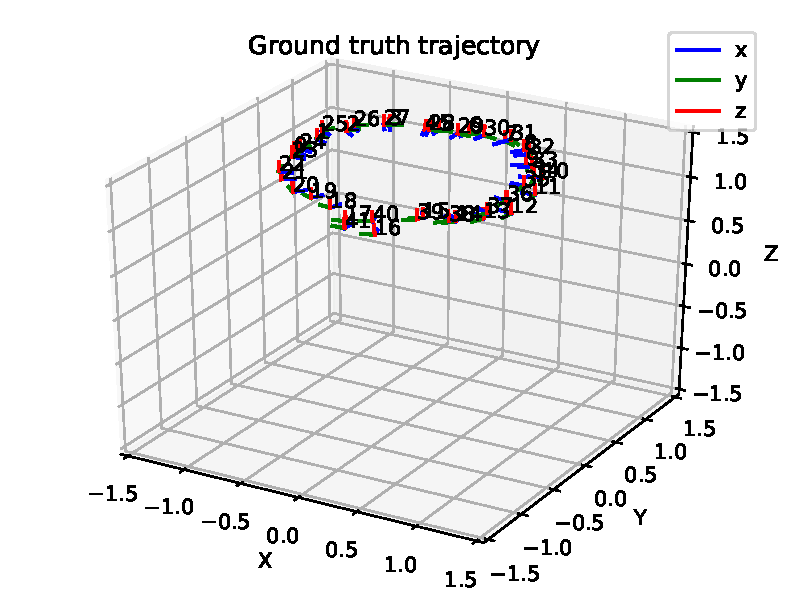
\includegraphics[width=80mm]{../quad/basic-reg-saves/50/atrj_gt.pdf}
        \caption{Ground truth trajectory (skip 50)}
      \end{subfigure} 
      \\
      \begin{subfigure}[t]{0.5\textwidth}
        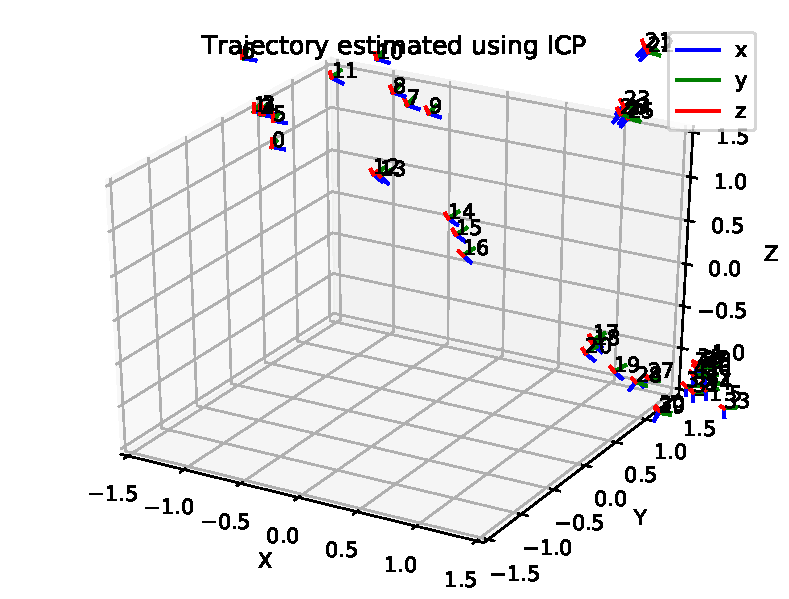
\includegraphics[width=80mm]{../quad/basic-reg-saves/50/atrj_icp.pdf}
        \caption{ICP absolute trajectory}
      \end{subfigure} %
      ~
      \begin{subfigure}[t]{0.5\textwidth}
      \centering
        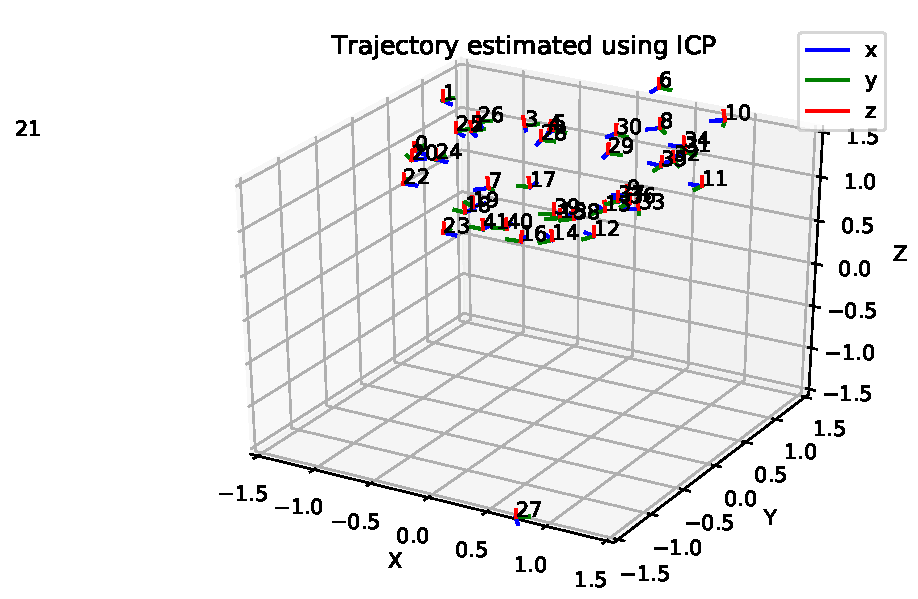
\includegraphics[width=80mm]{../quad/basic-reg-saves/50/rtrj_icp.pdf}
        \caption{ICP relative trajectory}
      \end{subfigure} 
      \caption{Trajectories for ICP on the quadcopter 1 dataset, with 50 frames skipped.}
      \label{f: quad3 trj}
    \end{figure}


\bibliographystyle{abbrvnat}
\bibliography{../Report/ENGN4217}

\end{document}